\section{Introduction}
\label{sec:intro}

This work contains a collection of applications of the 
Discrete Gauss-Bonnet theorem.
I hope that the number of examples continues to increase.
Please share any applications of the theorem that you feel
ought to  be included.


To warm up, let's consider a special case of the Gauss-Bonnet
theorem that the ready may already be familiar with.
\begin{theorem}\label{thm:triangle}
In the plane, the sum of the interior angles of a triangle is $\pi$.
\end{theorem}
\begin{proof}
Draw a line parallel to one edge through the opposite vertex.
By alternating interior angles in the plane, the sum of the angles
in the triangle equal  a straight line.
See \figref{angles} for on illustration. 



\begin{figure}[htb]
\centering
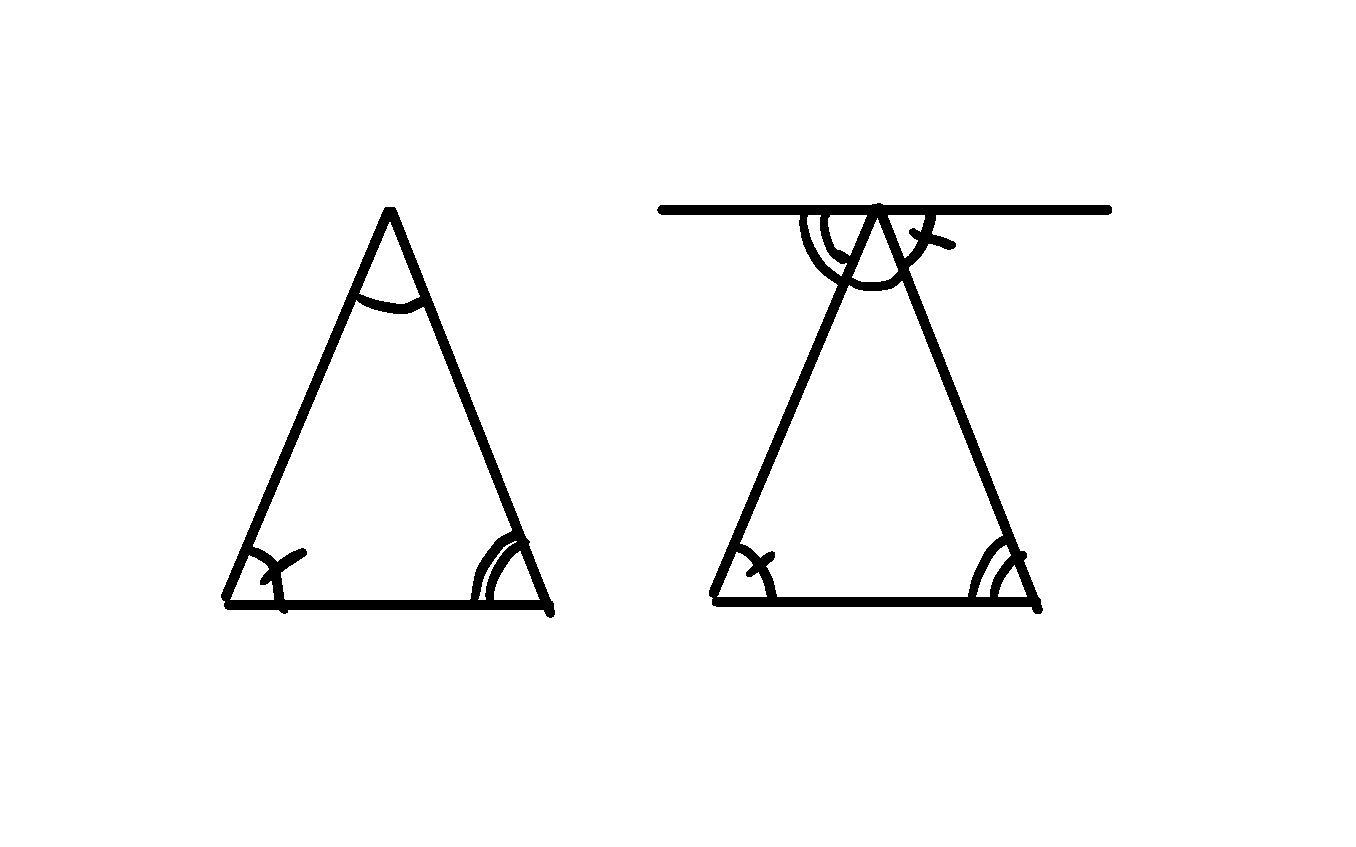
\includegraphics[width=.3\textwidth]{curvature/plane-case}
\caption{A proof that, in the plane, the sum of the angles of a triangle is $\pi$.}
\label{fig:angles}
\end{figure}

\end{proof}

This is remarkable because the sum of the angles of a triangle does not
depend on certain properties of the  triangle, such as the orientation in the plane or
the scale factor of the triangle.
We will see that more general versions of the Gauss-Bonnet theorem allow us 
to compute measurements independent of stretching and rotating.

But even this simple version of the theorem is useful.
Consider any simple polygon $P$ on $n$ vertices. 
What is the sum of the interior angles of $P$?
One could measure each angle, but if $n$ is large they would eventually
get tired.
Instead, we notice that any polygon with $n$ vertices can be
triangulated with $n-2$ triangles. This can be proved by induction.
Thus, when we traverse $P$ we go around $n-2$ triangles each contributing
$\pi$.
As a corollary to \thmref{triangle} we have
\begin{corollary}\label{cor:angles}
In the plane, any simple polygon $P$ with $n$ vertices,
the sum of the interior angles of $P$ is $(n-2)\pi$.

\end{corollary}






